\documentclass[12pt,a4paper,numbers=endperiod]{article}


%\usepackage[ngerman]{babel}
\usepackage[utf8]{inputenc}
\usepackage{amsmath}
\usepackage{amssymb}
\usepackage{amsfonts}
\usepackage{leftidx}
\usepackage{graphicx}
\usepackage{lipsum}                    
\usepackage{xargs} 
\usepackage{subfigure}
\usepackage{siunitx}
\usepackage{booktabs,caption}
\usepackage{float}
\usepackage{url}
\usepackage{mathrsfs}
\usepackage{titlesec}
\usepackage{tabularx}
\titlelabel{\thetitle. \,}
\usepackage{fancyhdr}
\pagestyle{fancy}
\usepackage[pdftex,dvipsnames]{xcolor}  % Coloured text etc.
% 
\usepackage[colorinlistoftodos,prependcaption,textsize=tiny]{todonotes}
\newcommandx{\unsure}[2][1=]{\todo[linecolor=red,backgroundcolor=red!25,bordercolor=red,#1]{#2}}
\newcommandx{\change}[2][1=]{\todo[linecolor=blue,backgroundcolor=blue!25,bordercolor=blue,#1]{#2}}
\newcommandx{\info}[2][1=]{\todo[linecolor=OliveGreen,backgroundcolor=OliveGreen!25,bordercolor=OliveGreen,#1]{#2}}
\newcommandx{\improvement}[2][1=]{\todo[linecolor=Plum,backgroundcolor=Plum!25,bordercolor=Plum,#1]{#2}}
\newcommandx{\thiswillnotshow}[2][1=]{\todo[disable,#1]{#2}}
%
%\fancyhf{}
%Customize Site header with discipline and report phase name
\fancyhead[L]{\small\sffamily Discipline}
\fancyhead[R]{\small\sffamily Project Karman}
\fancyhead[C]{\small\sffamily Report Name}
\newcommand{\RN}[1]{\uppercase\expandafter{\romannumeral#1}}
\newcommand{\im}{\mathrm{i}}
\newcommand{\expo}{\mathrm{e}}
\newcommand{\lf}{\left(}
\newcommand{\rt}{\right)}

\begin{document}

\begin{titlepage}
	\begin{center}
	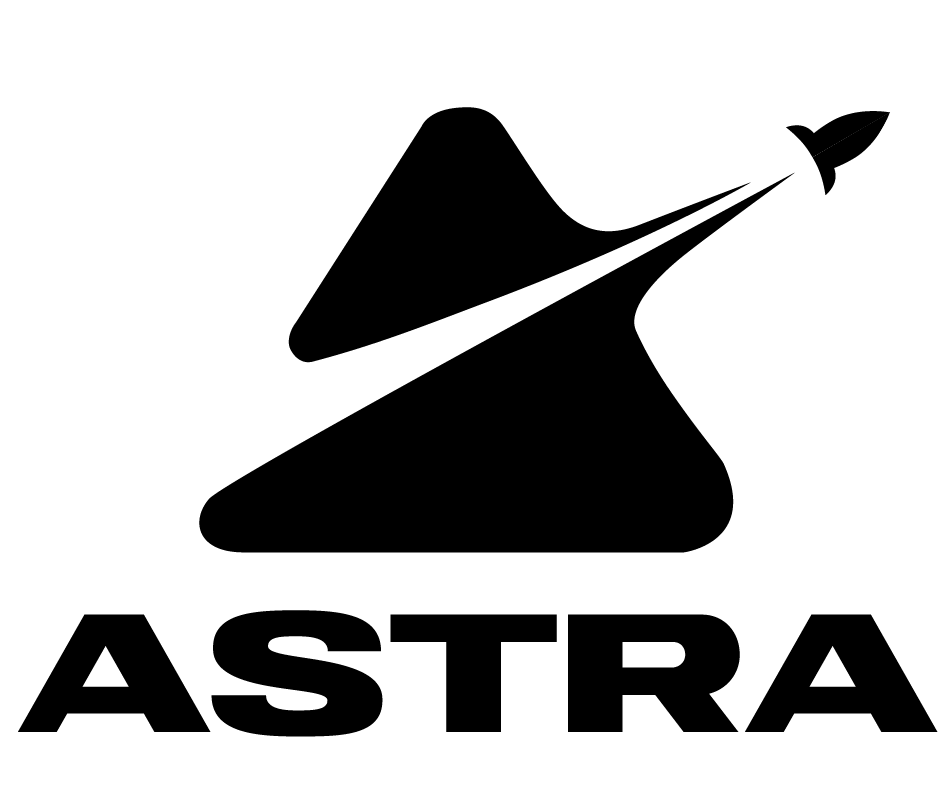
\includegraphics[width=0.5\textwidth]{Official_ASTRA_LOGO.png} \par \vspace{1cm}
	{\LARGE \bf Association for Space Technology and Research Applications }
	\par \vspace{0.5cm}	
	{\line(1,0){350}}
	\par \vspace{-1.5cm}
	
\includegraphics[width=0.7\textwidth]{Project_Karman_Logo.png}
	\par \vspace{-2cm}
	{\LARGE \bf Project Karman}\\
	\vspace{0.5cm}
	{\line(1,0){350}}
	\par \vspace{0.5cm}
	%customize Phase report and Discipline title here
	{\Large \bf Test Report - Avionics System}

	%write report date

	\end{center}
\end{titlepage}
%page with member names
\noindent
\thispagestyle{empty}
	\par \vspace{0.5cm}
{\Large \bf Document number:}\\
\par \vspace{0.3cm}
{\Large \bf Issued:}\\
\par \vspace{0.3cm}
{\Large \bf Revision:}\\
\par \vspace{0.3cm}	
{\Large \bf Prepared:}\\
\par \vspace{0.3cm}
{\Large \bf Released:}\\
\par \vspace{0.5cm}
{\Huge \bf Team Members}\\
 \\
1.\\
2.\\
3.\\
4.\\
5.\\
6.\\
7.\\
\vspace*{\fill} \\
Date of Submission:
\newpage

%make table of contents, list of figures and table in document automatically
\tableofcontents
\newpage

\listoffigures
\listoftables
\newpage

\section{Summary}
\subsection{Scope}
This document describes the ------ test procedure for the --- of the --- unit to meet the requirements --- and ---.\\
Purpose of the test is to demonstrate that -----.\\
This document establishes the test procedure as well as the test sequence required for the --- test of the --- unit.\\
\subsection{Test Objectives}
The major test objectives are:\\
1. To demonstrate that the -- unit adequately meets the --- requirements.\\
2. To ensure/demonstrate that --- unit can be operated in --- mode.
\subsection{Test Specimen}
A list of the test specimen parts is given in the table below.
\begin{table}[H]
	\centering
	\caption{Test Specimen}
	\begin{tabular}{lll}
		\toprule
	Test item & Hardware/Part number & Model \\
	\midrule
	--Unit & 88888 & ABC-X \\
	--Unit & 99999 & XYZ-S\\
		\bottomrule
\end{tabular}
\label{t:specimen}
\end{table}

\subsection{Test Verification Matrix}
\begin{table}[H]
	\centering
	\caption{Test Verification Matrix}
	\begin{tabular}{llll}
			\toprule
		Test Requirement & & Test Temperatures & Remarks\\
		\midrule
		Performance Test & AV001 & +X\si{deg}, -X\si{deg} & Acceptance level\\
		\bottomrule
	\end{tabular}
\label{t:VerifMatrix}
\end{table}

\newpage
\section{References}
\subsection{Applicable Documents}
AV-COM-SPEC-777    \quad ABC-Band RF Specification\\ 
AV-GPS-SPEC-777   \quad GPS -- Specification
\subsection{Reference Documents}
\
\subsection{Abbreviations}
\newpage
\section{Test Setup}
The general setup to test --- of the -- unit is shown in the figure below.
\newpage
\section{Test Conditions}
This section defines the general conditions under which the test shall be carried out.
\subsection{Responsibilities}
The test shall be performed under the supervision of the Test Review Board (TRB) consisting of the following members:
\par \vspace{0.3cm}
{\bf---- Team Lead:}\\
- Operation of measuring instrumentation and test facility\\
- Performance of functional checks\\
- Compilation of test results\\
- General safety precautions\\
- Test evaluation\\

{\bf External Review Board member:}\\


{\bf External Safety Assurance Engineer:}\\ 

\subsection{Test Reviews}
The Critical Design Review (CDR) and the XYZ Review shall be conducted by the External Test Review Board. 
\subsection{Environmental Conditions}
\begin{table}[H]
	\centering
	\caption{Environmental Conditions}
\begin{tabular}{llll}
	\toprule
	Conditions & Requirements & Verification\\
	\midrule
	Tempearture & +22 degrees & Thermometer \\
	Relative Humidity & 50\% & Hygrometer\\
	Pressure & 110bar & xy gauge \\
	\bottomrule
\end{tabular}
\label{t:Env_Cond}
\end{table}
	
	 

\subsection{Test Tolerances}
\begin{table}[H]
	\centering
	\caption{Test Tolerances}
	\begin{tabular}{lll}
		\toprule
		Parameter & Tolerance Allowed & Comment\\
		\midrule
		Voltage & +/- 1 \% & xxx\\
		Current & +/- 1 \% & N/A\\
	Frequency & +/1 ppm & ECSS-x-x \\
		\bottomrule
	\end{tabular}
	\label{t:Tolerance}
\end{table}

\subsection{Instrumentation and Test Equipment}
\subsection{Test Safety Precautions}
Handle xyz with care.\\
Be aware of xxx changes during the process of xxx.\\
Strong precautions need to be taken for xxx.
\newpage
\section{Test Program}
\subsection{Test Criteria}
The performance mentioned has to be in line with the relevant requirement specification defined within [PR005]. (PR005: Unit 4)
\subsection{Test Success Criteria}
The acceptance tests are considered to be successful if the following criteria are fulfilled:\\
- No visible damage has occurred. \\ 
- All tested parameters are within specified limits.\\
- No NCR was raised. (Signs of non-conformity raised by someone who inspected the units)

\subsection{Recorded Data}
All actions and results a shall be documented in the test report.\\
The following data shall be measured and recorded:\\
- Picture of the set-up.\\
- Picture of the test-specimen connected to the measurement equipment.\\
- All measurement data has to be written in the results sheet (chapter 6).\\
Anomalies, deficiencies or ambiguities are to be immediately reported and mentioned in the Problem-Failure report. Any variation to the test procedure has to be discussed and approved.\\
Any deviation and malfunction has to be mentioned in the Non-conformance report.\\
An overview of the general test sequence is shown in Figure below.

\subsection{Vibration test}
18 seconds cycles (sinusoidal and random).\\
Frequencies (rocket engine): 100Hz-5000Hz.\\
100, 250, 750, 1000, 2000, 3000, 4000, 5000. (times 5)\\
Random(100-5000Hz): Also 5 times.\\
Amplitudes: \\
Avionics bay dimensions: (model) (diagram with description) (2D drawing with dimensions) \\
Connectors: \\



\subsection{Test Descriptions}
\newpage
\section{Test Result Sheets}

\noindent
Include, plots, checklists, tables and pictures here.\\
Also include an Annex of used equipment, Procedure variation sheet, Non-conformity report, Problem-failure report.
\begin{figure}[H]
\centering
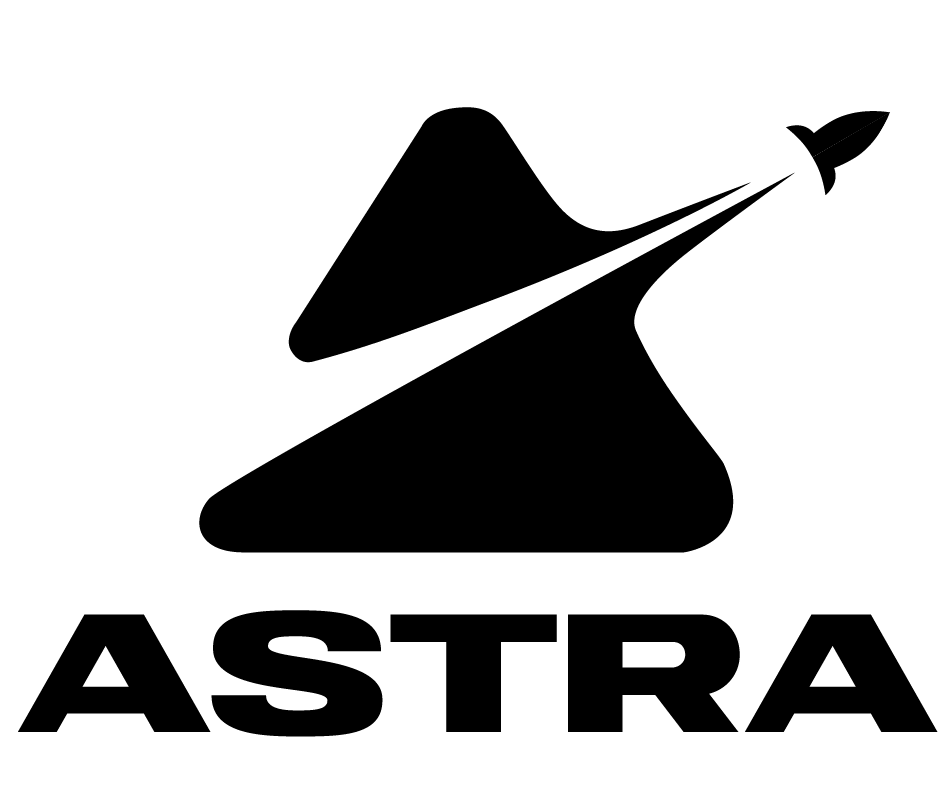
\includegraphics[width=0.3\textwidth]{Official_ASTRA_LOGO.png}
\caption{LOGO of ASTRA}
\label{logo}
\end{figure}

\end{document}













